%%%%%%%%%%%%%%%%%%%%%%%%%%%%%%%%%%%%%%%%%
% Short Sectioned Assignment
% LaTeX Template
% Version 1.0 (5/5/12)
%
% This template has been downloaded from:
% http://www.LaTeXTemplates.com
%
% Original author:
% Frits Wenneker (http://www.howtotex.com)
%
% License:
% CC BY-NC-SA 3.0 (http://creativecommons.org/licenses/by-nc-sa/3.0/)
%
%%%%%%%%%%%%%%%%%%%%%%%%%%%%%%%%%%%%%%%%%

%----------------------------------------------------------------------------------------
%	PACKAGES AND OTHER DOCUMENT CONFIGURATIONS
%----------------------------------------------------------------------------------------

\documentclass[paper=a4, fontsize=11pt]{scrartcl} % A4 paper and 11pt font size

\usepackage[T1]{fontenc} % Use 8-bit encoding that has 256 glyphs
\usepackage{fourier} % Use the Adobe Utopia font for the document - comment this line to return to the LaTeX default
\usepackage[english]{babel} % English language/hyphenation
\usepackage{amsmath,amsfonts,amsthm} % Math packages

\usepackage{graphicx}
\usepackage{float}

\usepackage{sectsty} % Allows customizing section commands
\allsectionsfont{\normalfont\scshape} % Make all sections centered, the default font and small caps

\usepackage{fancyhdr} % Custom headers and footers
\pagestyle{fancyplain} % Makes all pages in the document conform to the custom headers and footers
\fancyhead{} % No page header - if you want one, create it in the same way as the footers below
\fancyfoot[L]{} % Empty left footer
\fancyfoot[C]{} % Empty center footer
\fancyfoot[R]{\thepage} % Page numbering for right footer
\renewcommand{\headrulewidth}{0pt} % Remove header underlines
\renewcommand{\footrulewidth}{0pt} % Remove footer underlines
\setlength{\headheight}{13.6pt} % Customize the height of the header

\numberwithin{equation}{section} % Number equations within sections (i.e. 1.1, 1.2, 2.1, 2.2 instead of 1, 2, 3, 4)
\numberwithin{figure}{section} % Number figures within sections (i.e. 1.1, 1.2, 2.1, 2.2 instead of 1, 2, 3, 4)
\numberwithin{table}{section} % Number tables within sections (i.e. 1.1, 1.2, 2.1, 2.2 instead of 1, 2, 3, 4)

\setlength\parindent{0pt} % Removes all indentation from paragraphs - comment this line for an assignment with lots of text

%----------------------------------------------------------------------------------------
%	TITLE SECTION
%----------------------------------------------------------------------------------------

\newcommand{\horrule}[1]{\rule{\linewidth}{#1}} % Create horizontal rule command with 1 argument of height

\title{	
\normalfont \normalsize 
\textsc{BRSU} \\ [25pt] % Your university, school and/or department name(s)
\horrule{0.5pt} \\[0.4cm] % Thin top horizontal rule
\huge Homework for Artificial Intelligence for Robotics\\Assignment 9 \\ % The assignment title
\horrule{2pt} \\[0.5cm] % Thick bottom horizontal rule
}

\author{Bastian Lang} % Your name

\date{\normalsize\today} % Today's date or a custom date

\begin{document}

\maketitle % Print the title


\section{Practical Part}

\subsection{Task}
Given an initial location and a set of locations and time deadlines to reach those locations, implement an algorithm that finds a path that reaches every location within the given time deadline.\\
The locations for a single problem are stored in a text file. There are five different scenarios, i.e. there are five text files.\\
Use three different strategies for picking the next city:
\begin{itemize}
\item ordered by line number in provided file
\item ordered by euclidean distance
\item ordered by deadline
\end{itemize}


\subsection{Approach}
I chose a recursive approach. Starting with the initial city as the current city, I pass the fringe (list of cities left) and an empty list for the path taken so far as parameters into my recursive function.\\
In this function I first calculate the time needed for the whole path taken so far and check if the deadline for the current element is fulfilled. I then sort the fringe according to the strategy and for every city left in the fringe I call the function again. This time with the fringe reduced by the chosen next element and the current path extended by the current element. The function directly returns if a solution is found and does not check the remaining cities. If for one function call the fringe is empty and the time deadline for the current element is fulfilled, a solution is found and returned.


\subsection{Result}
\begin{itemize}
\item Of the five given scenarios, four are solvable.
\item Using euclidean distance always takes the least number of expansions, line numbering always the most.
\item The length of the resulting path is always shortest or as short as the others for the euclidean distance.
\item If a problem is not solvable at all, all strategies expand the whole search space.
\end{itemize}

\subsubsection{Scenario 1}
\begin{tabular}{|c|c|c|}
\hline 
 & Time Taken & \# Expansions \\ 
\hline 
Line Numbers & 65.8426459044 & 306 \\ 
\hline 
Euclidean distance & 65.8426459044 & 38 \\ 
\hline 
Remaining deadline & 65.8426459044 & 88 \\ 
\hline 
\end{tabular} 


\subsubsection{Scenario 2}
\begin{tabular}{|c|c|c|}
\hline 
 & Time Taken & \# Expansions \\ 
\hline 
Line Numbers & 90.4324507719 & 157216 \\ 
\hline 
Euclidean distance & 82.7338754883 & 38 \\ 
\hline 
Remaining deadline & 105.930512517 & 60123 \\ 
\hline 
\end{tabular} 


\subsubsection{Scenario 3}
\begin{tabular}{|c|c|c|}
\hline 
 & Time Taken & \# Expansions \\ 
\hline 
Line Numbers & 75.1388213649 & 2995 \\ 
\hline 
Euclidean distance & 74.2638321331 & 119 \\ 
\hline 
Remaining deadline & 75.1388213649 & 5707 \\ 
\hline 
\end{tabular} 


\subsubsection{Scenario 4}
Not solvable\\

\begin{tabular}{|c|c|c|}
\hline 
 & Time Taken & \# Expansions \\ 
\hline 
Line Numbers & N/A & 325656 \\ 
\hline 
Euclidean distance & N/A & 325656 \\ 
\hline 
Remaining deadline & N/A & 325656 \\ 
\hline 
\end{tabular} 

\subsubsection{Scenario 5}
\begin{tabular}{|c|c|c|}
\hline 
 & Time Taken & \# Expansions \\ 
\hline 
Line Numbers & 194.889517611 & 608395 \\ 
\hline 
Euclidean distance & 97.267315083 & 17 \\ 
\hline 
Remaining deadline & 234.249535637 & 127 \\ 
\hline 
\end{tabular} 



\subsubsection{Plots}

\begin{figure}[H]
	\centering
  	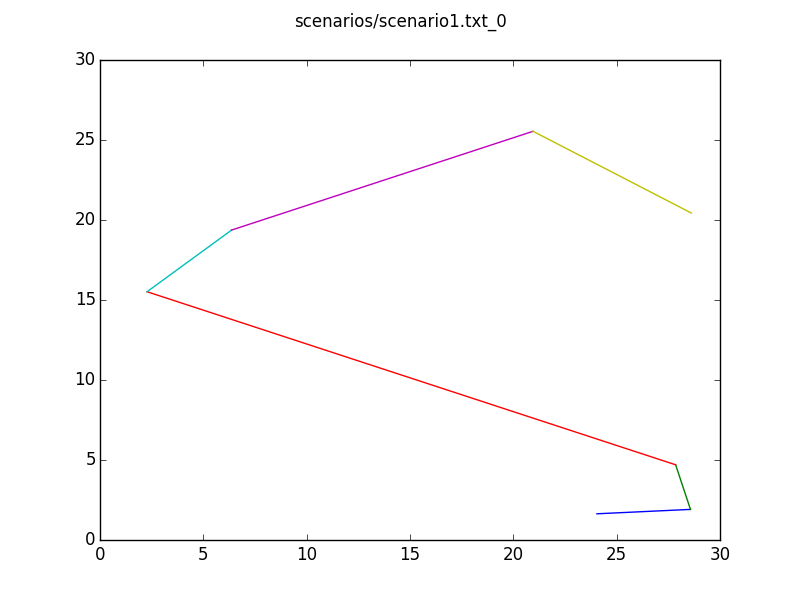
\includegraphics[width=1\textwidth]{results/1_0.png}
	\caption{Path for scenario 1, line numbering}
\end{figure}
\begin{figure}[H]
	\centering
  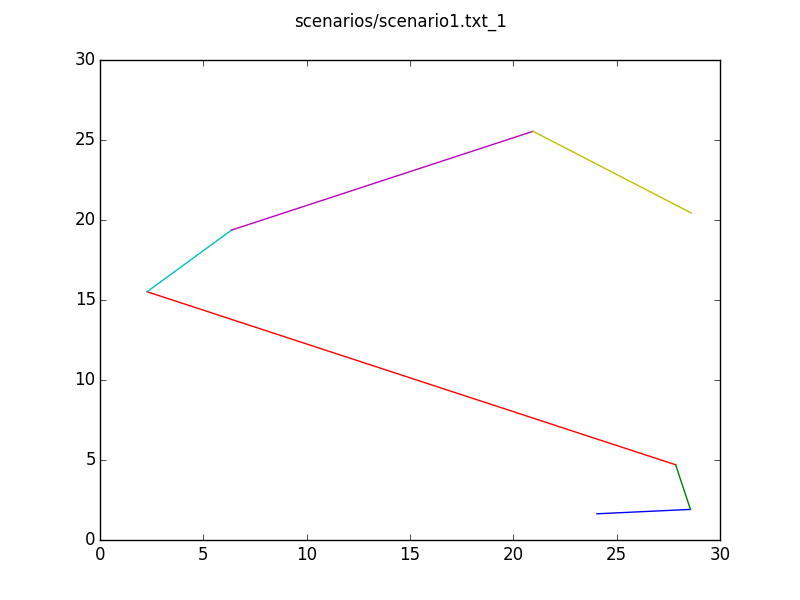
\includegraphics[width=1\textwidth]{results/1_1.png}
	\caption{Path for scenario 1, euclidean distance}
\end{figure}
\begin{figure}[H]
	\centering
  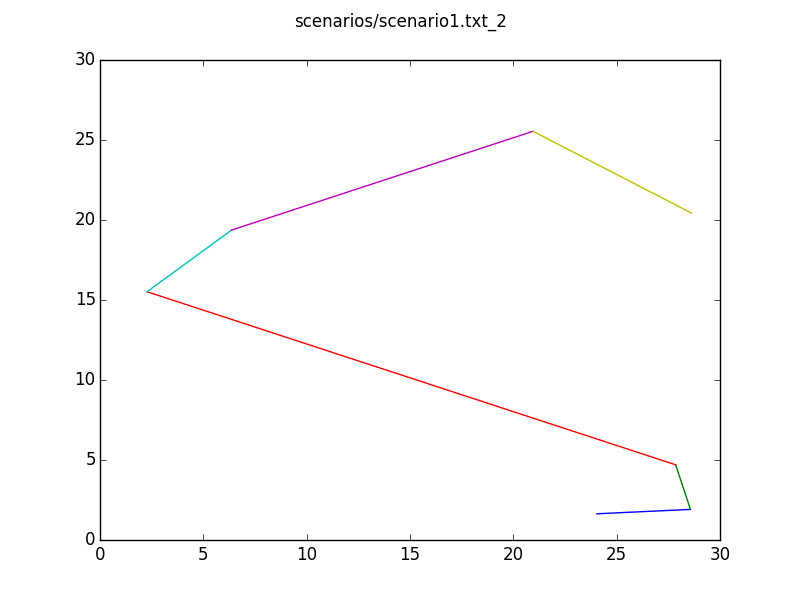
\includegraphics[width=1\textwidth]{results/1_2.png}
	\caption{Path for scenario 1, deadline}
\end{figure}

\begin{figure}[H]
	\centering
  	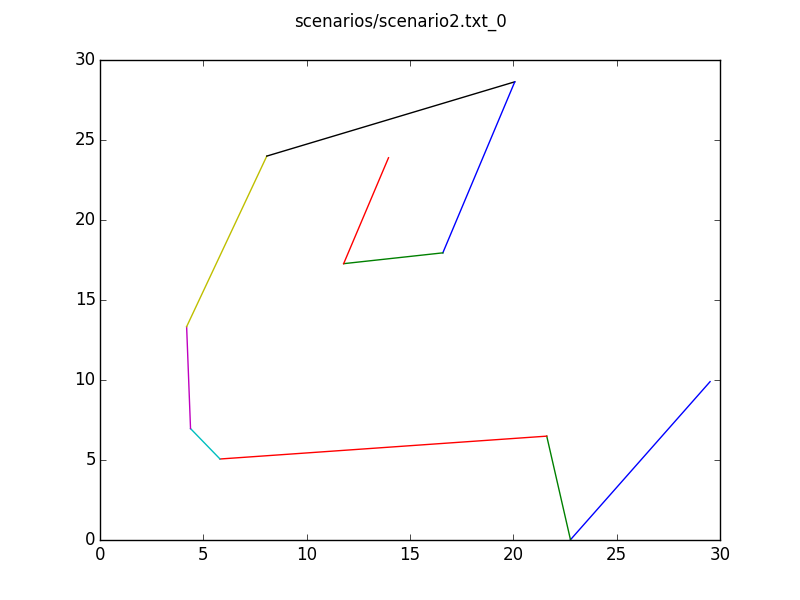
\includegraphics[width=1\textwidth]{results/2_0.png}
	\caption{Path for scenario 2, line numbering}
\end{figure}
\begin{figure}[H]
	\centering
  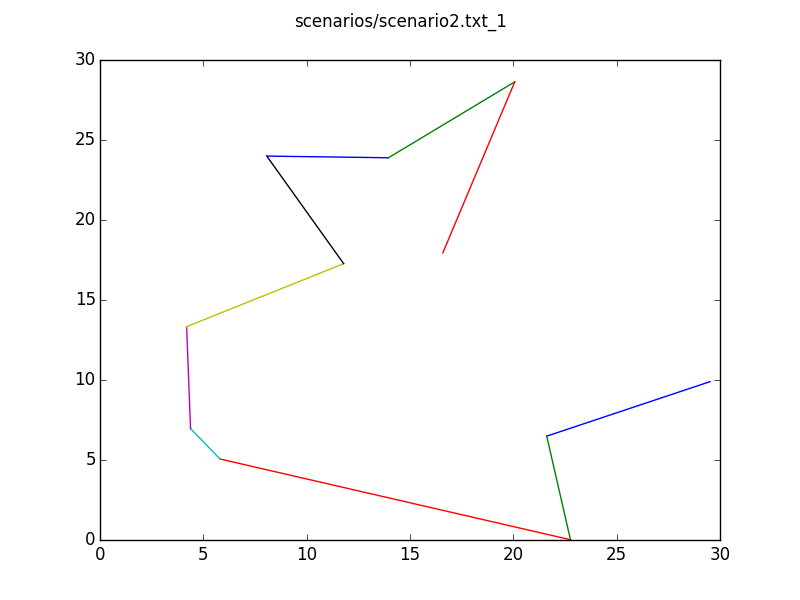
\includegraphics[width=1\textwidth]{results/2_1.png}
	\caption{Path for scenario 2, euclidean distance}
\end{figure}
\begin{figure}[H]
	\centering
  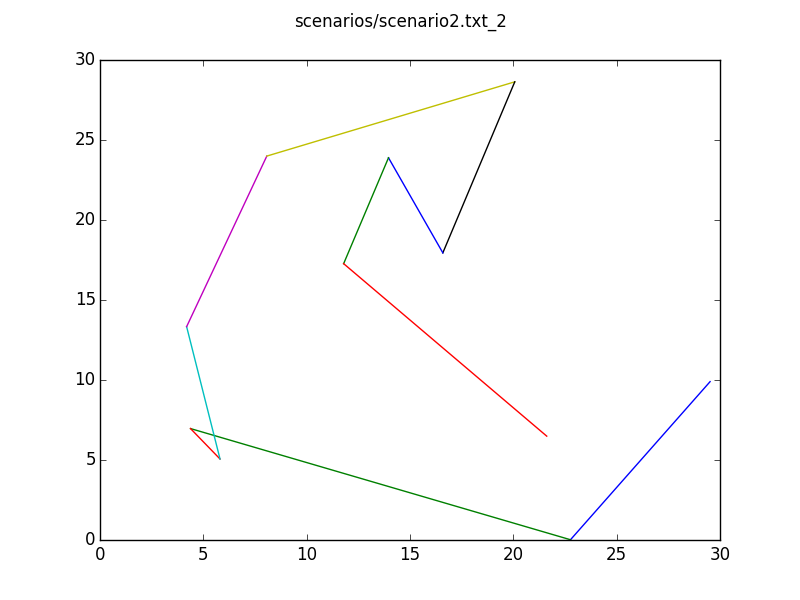
\includegraphics[width=1\textwidth]{results/2_2.png}
	\caption{Path for scenario 2, deadline}
\end{figure}

\begin{figure}[H]
	\centering
  	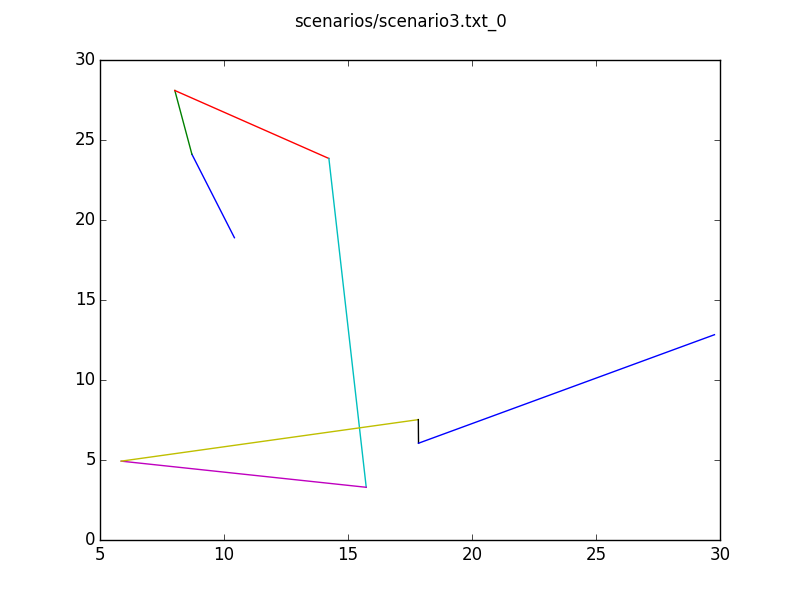
\includegraphics[width=1\textwidth]{results/3_0.png}
	\caption{Path for scenario 3, line numbering}
\end{figure}
\begin{figure}[H]
	\centering
  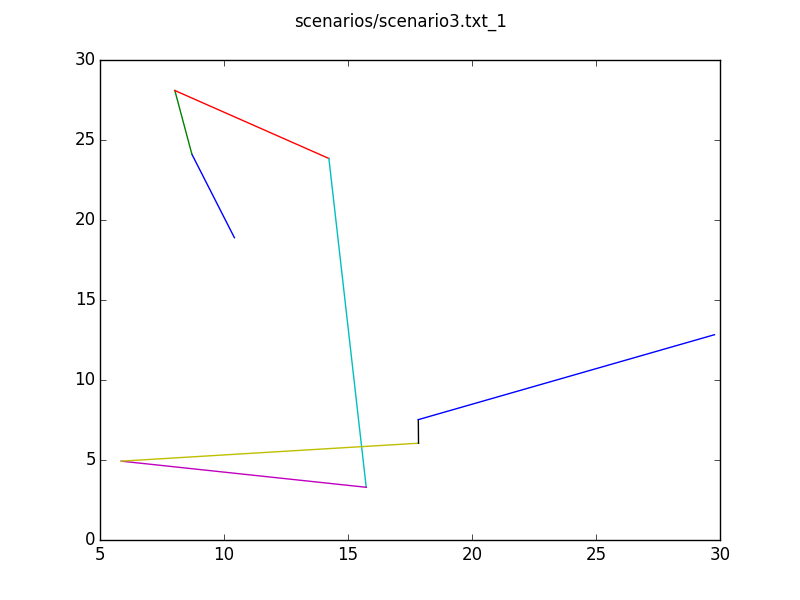
\includegraphics[width=1\textwidth]{results/3_1.png}
	\caption{Path for scenario 3, euclidean distance}
\end{figure}
\begin{figure}[H]
	\centering
  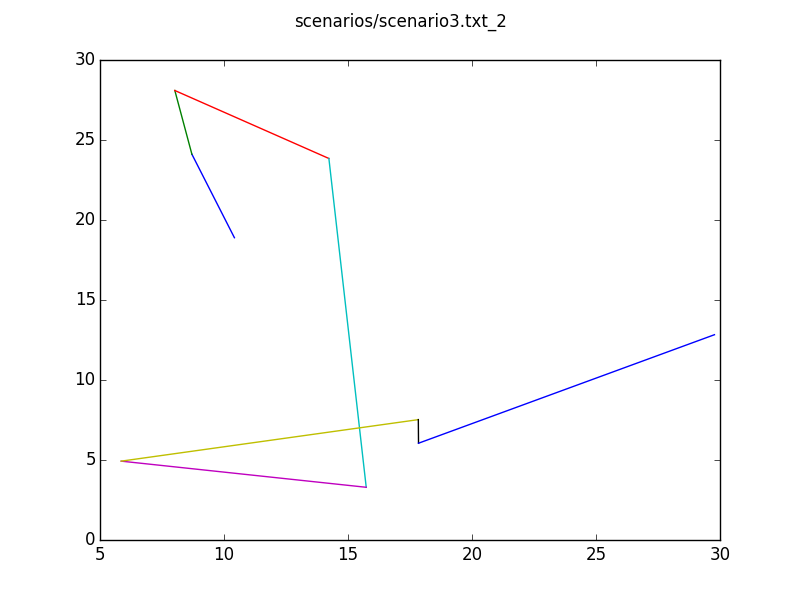
\includegraphics[width=1\textwidth]{results/3_2.png}
	\caption{Path for scenario 3, deadline}
\end{figure}

\begin{figure}[H]
	\centering
  	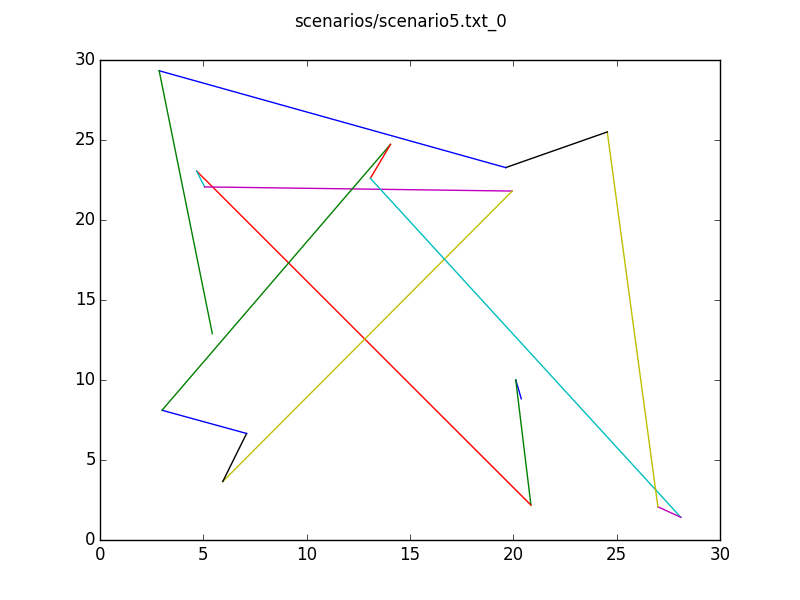
\includegraphics[width=1\textwidth]{results/5_0.png}
	\caption{Path for scenario 5, line numbering}
\end{figure}
\begin{figure}[H]
	\centering
  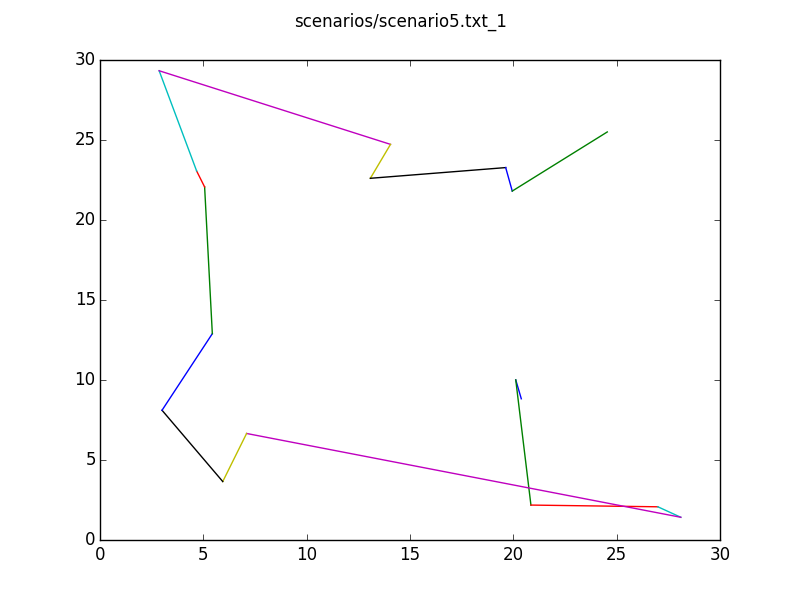
\includegraphics[width=1\textwidth]{results/5_1.png}
	\caption{Path for scenario 5, euclidean distance}
\end{figure}
\begin{figure}[H]
	\centering
  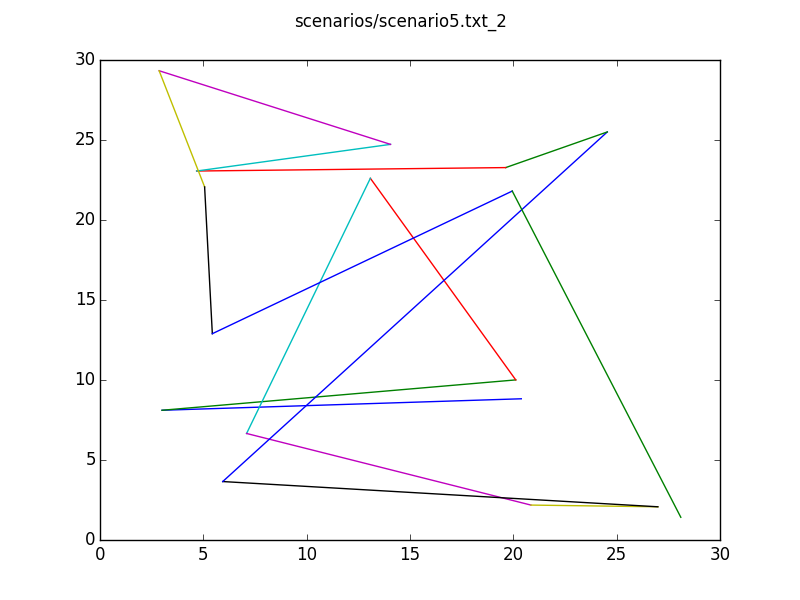
\includegraphics[width=1\textwidth]{results/5_2.png}
	\caption{Path for scenario5, deadline}
\end{figure}


\end{document}